\thispagestyle{fancy}
\vspace*{40 pt}
\subsection{Tela comando alimentação}
 Esta tela é acessada pelo botão "\textgreater" no menu superior esquerdo da tela de comando de máquina, pelo botão "\textless{}" no menu superior esquerdo da tela 
 comando impressoras ou impressora 1, pelo botão "ALM" em qualquer tela de comando e pelo botão comando da tela ajustes alimentação. A partir desta os botões "comando" 
 e "ajustes" começam a se comportar de maneira contextual de maneira que eles vão levar a tela correspondente a tela selecionada. Caso você já esteje na tela selecionada 
 você será levado a tela anterior.
 \vspace*{\fill}
\begin{figure}[h]
  \centering
  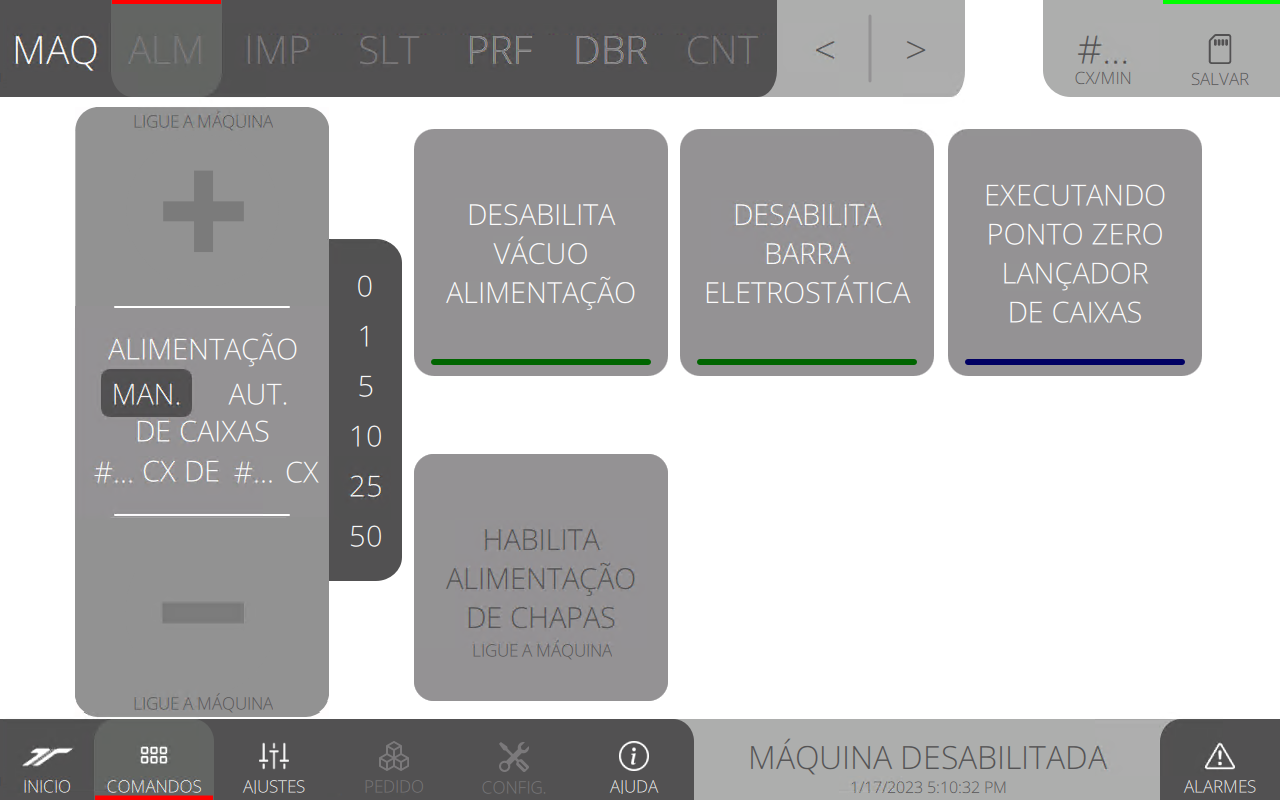
\includegraphics[width=576px,height=360px]{src/imagesFlexo/03-feeder/commands/e-Tela-Principal.png}
\end{figure}
\vspace*{\fill}

\newpage
\thispagestyle{fancy}
\vspace*{40 pt}
\subsubsection{\small{Configuração de alimentação de caixas modo manual}}
\vspace*{\fill}
\begin{figure}[h]
  \centering
  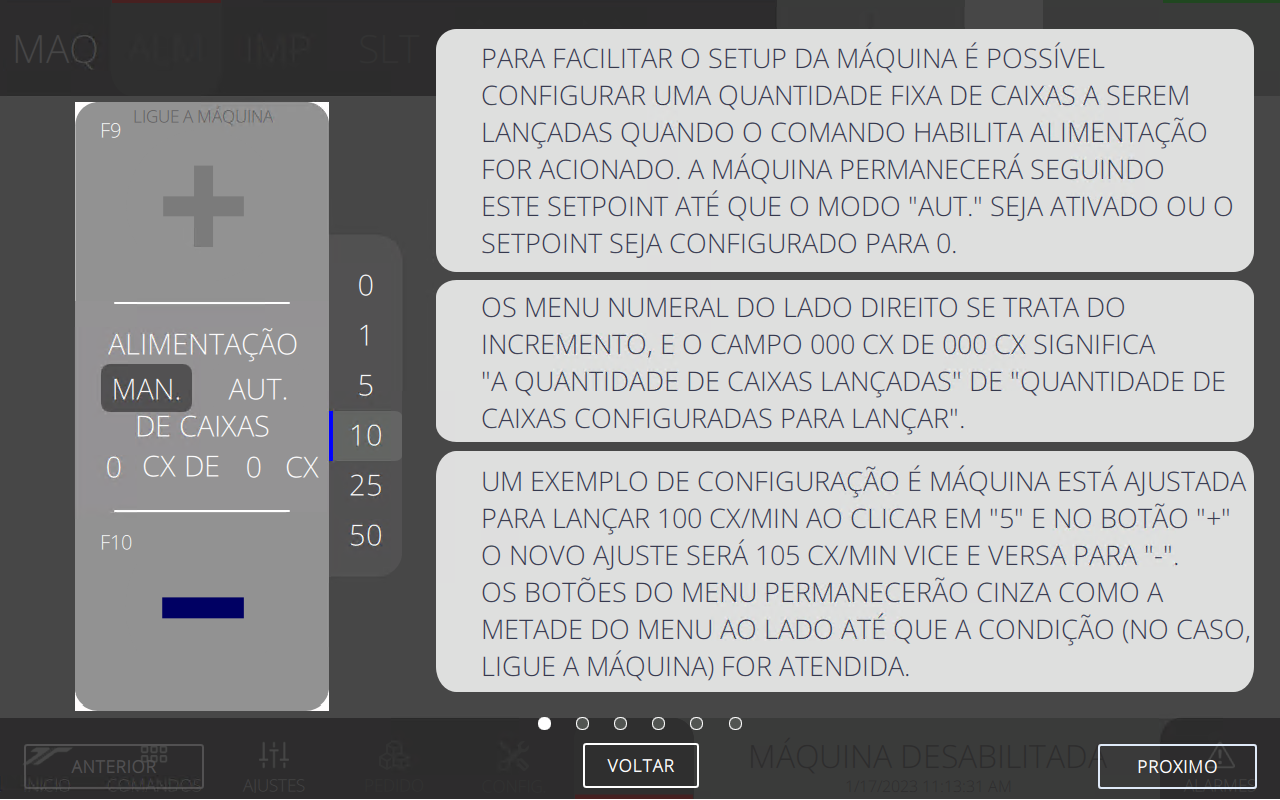
\includegraphics[width=576px,height=360px]{src/imagesFlexo/03-feeder/commands/e-1.png}
\end{figure}
\vspace*{\fill}


\newpage
\thispagestyle{fancy}
\vspace*{40 pt}
\subsubsection{\small{Configuração de alimentação de caixas modo automático}}
\vspace*{\fill}
\begin{figure}[h]
  \centering
  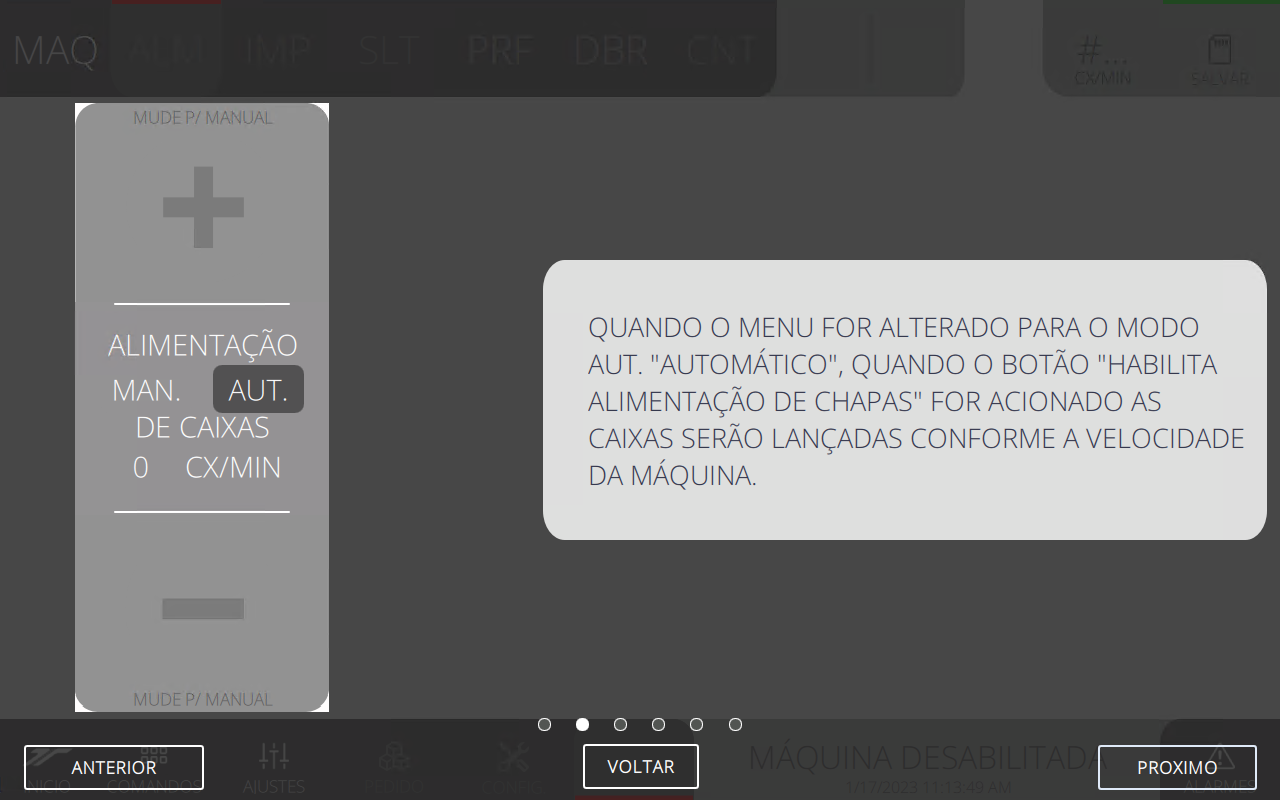
\includegraphics[width=576px,height=360px]{src/imagesFlexo/03-feeder/commands/e-2.png}
\end{figure}
\vspace*{\fill}

\newpage
\thispagestyle{fancy}
\vspace*{40 pt}
\subsubsection{\small{Habilita vácuo alimentação}}
\vspace*{\fill}
\begin{figure}[h]
  \centering
  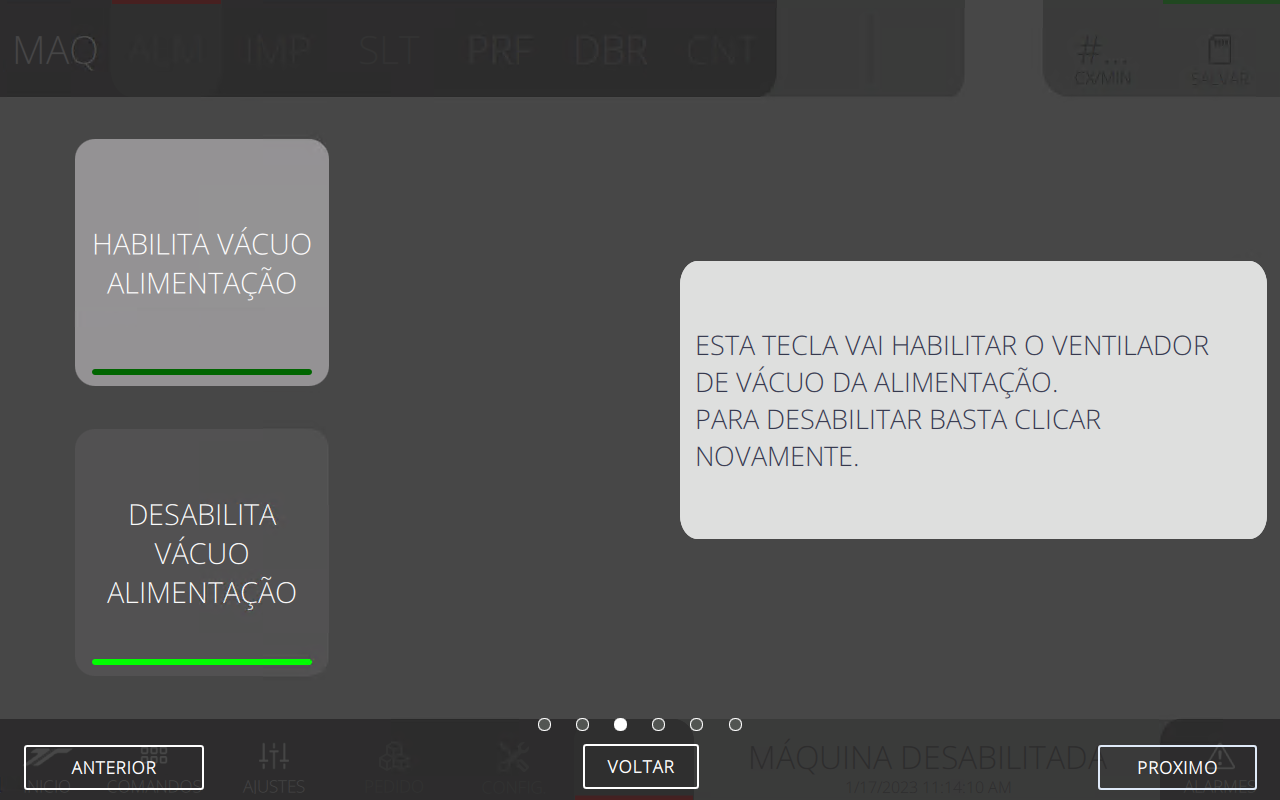
\includegraphics[width=576px,height=360px]{src/imagesFlexo/03-feeder/commands/e-3.png}
\end{figure}
\vspace*{\fill}

\newpage
\thispagestyle{fancy}
\vspace*{40 pt}
\subsubsection{\small{Executa ponto zero lançador de caixas}}
\vspace*{\fill}
\begin{figure}[h]
  \centering
  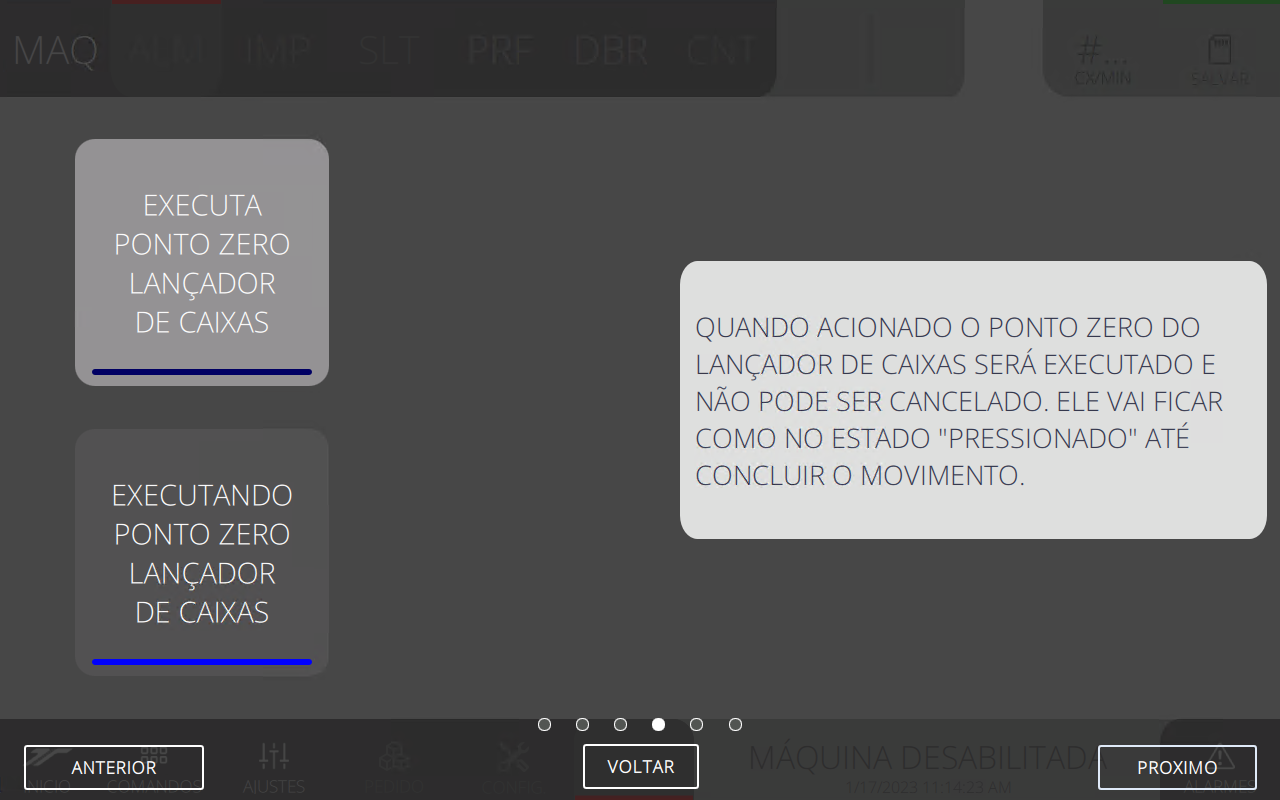
\includegraphics[width=576px,height=360px]{src/imagesFlexo/03-feeder/commands/e-4.png}
\end{figure}
\vspace*{\fill}

\newpage
\thispagestyle{fancy}
\vspace*{40 pt}
\subsubsection{\small{Habilita alimentação de chapas}}
\vspace*{\fill}
\begin{figure}[h]
  \centering
  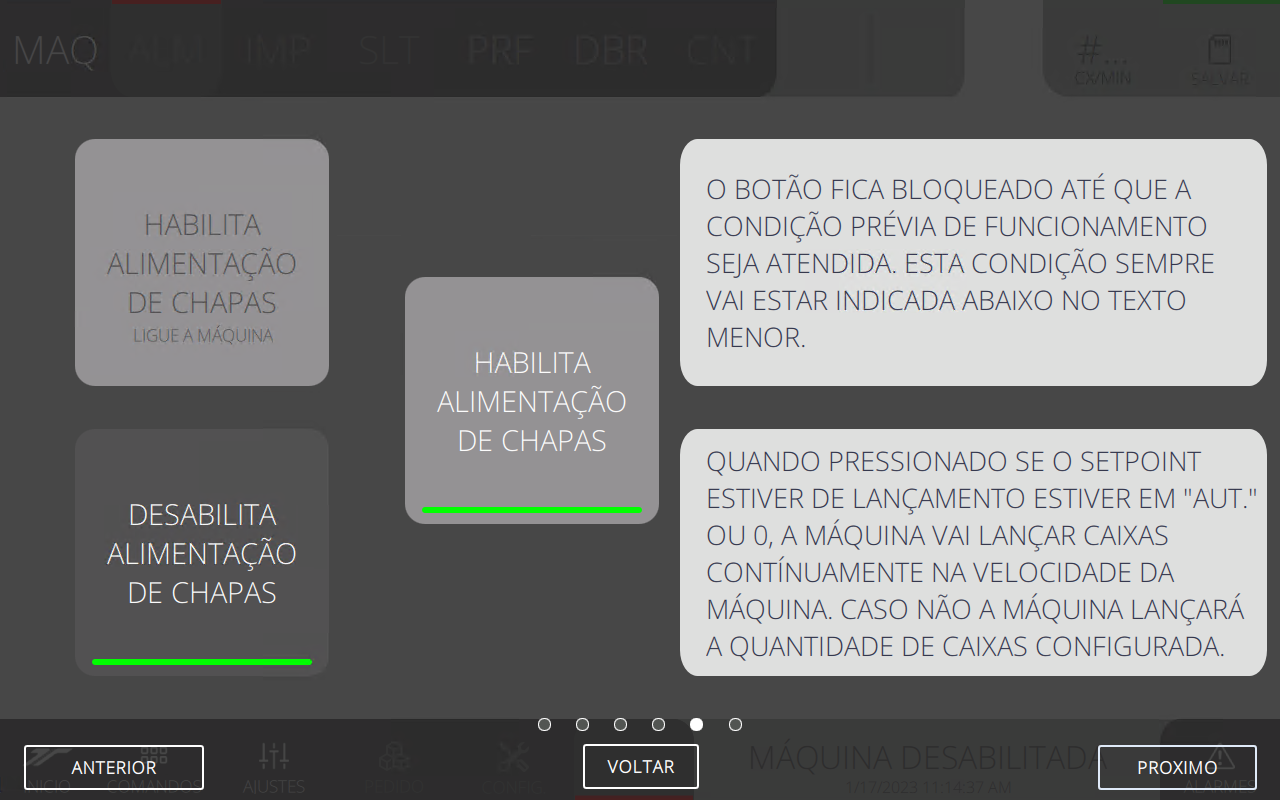
\includegraphics[width=576px,height=360px]{src/imagesFlexo/03-feeder/commands/e-5.png}
\end{figure}
\vspace*{\fill}

\newpage
\thispagestyle{fancy}
\vspace*{40 pt}
\subsubsection{\small{Habilita barra eletrostática}}
\vspace*{\fill}
\begin{figure}[h]
  \centering
  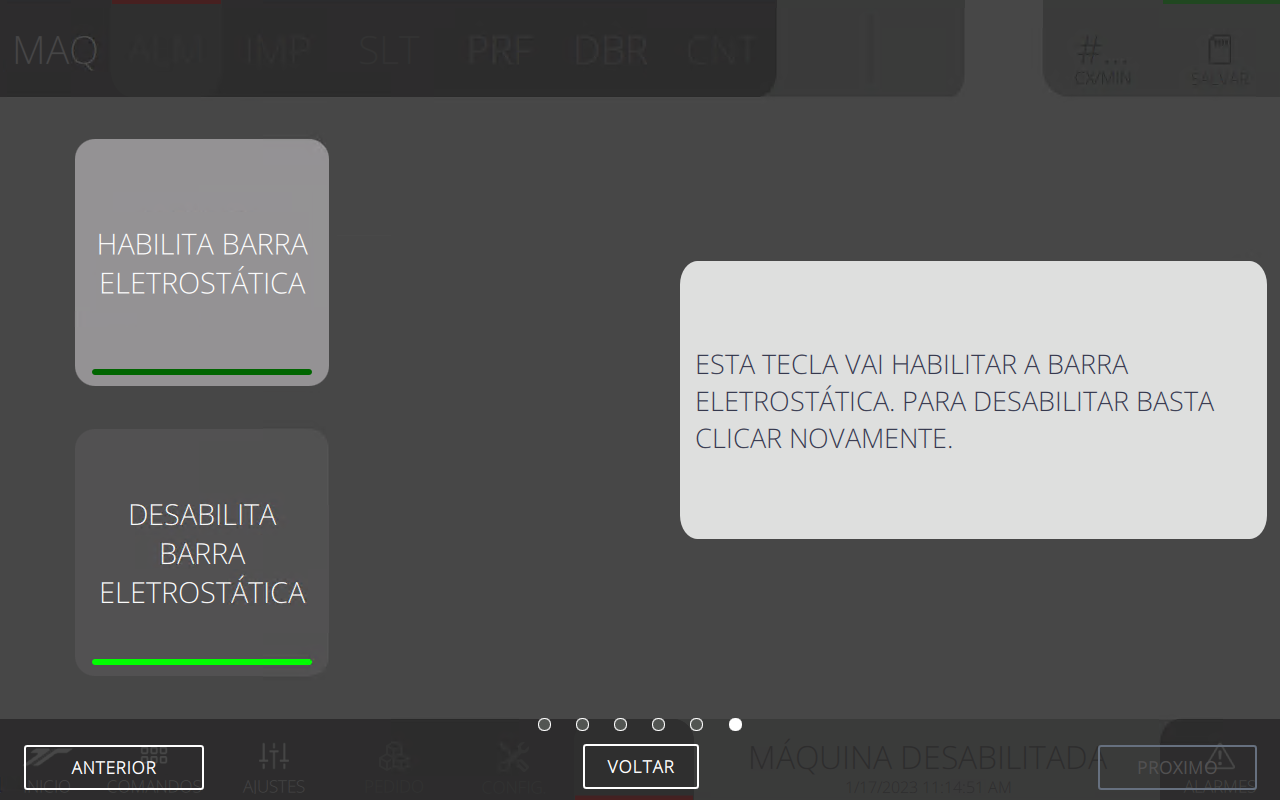
\includegraphics[width=576px,height=360px]{src/imagesFlexo/03-feeder/commands/e-6.png}
\end{figure}
\vspace*{\fill}